% ============================================================
% Capítulo: Diseño y Arquitectura del Sistema (Bloque B.8)
% ============================================================
\chapter{Diseño y arquitectura del sistema}
\label{cap:diseno-arquitectura}

El modelo arquitectónico de SGB-SaaS, aplicando el modelo C4 descrito
en la \autoref{sec:mt-c4}, está versionado como código fuente
en \texttt{docs/arquitectura/workspace.dsl} (Structurizr DSL, modelo
C4), en sus tres niveles completos -- Contexto, Contenedores y
Componentes -- que reemplazan los diagramas estáticos sin fuente
versionada de la Entrega~1A
(\texttt{docs/diagramas/diagrama\_c4\_capa1.png},
\texttt{diagrama\_c4\_capa2.jpeg}). Esos dos archivos permanecen
versionados en el repositorio como evidencia histórica del diseño
original, pero ya no se reproducen en este documento porque estaban
desactualizados (citaban \texttt{Google Books API} como sistema
externo, sin integración real en el código, y el segundo no incluía el
contenedor Redis). Las figuras siguientes son la exportación real y
automática de \texttt{workspace.dsl} con Structurizr
(\autoref{sec:c4-exportacion}), no una reconstrucción manual.

\begin{figure}[h]
\centering
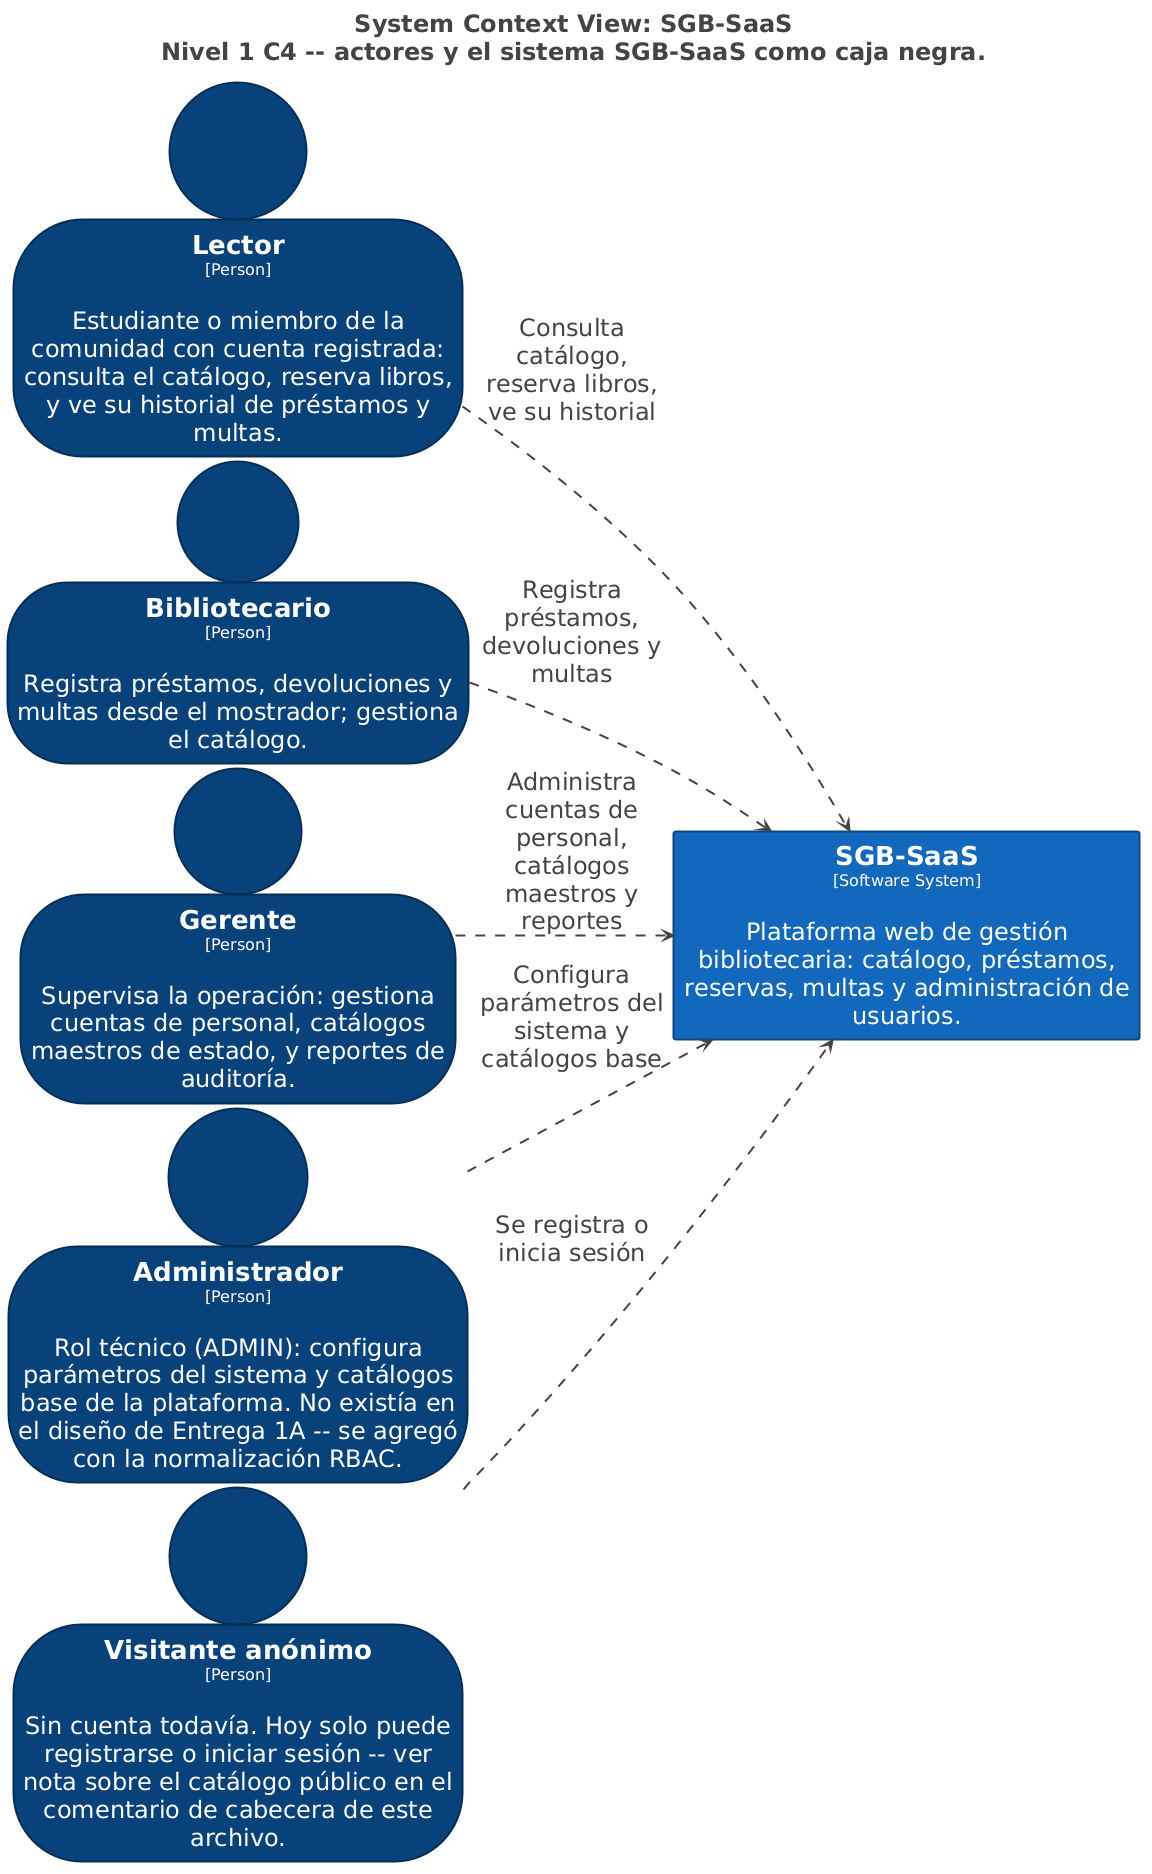
\includegraphics[width=0.85\textwidth]{arquitectura/c4-nivel1-contexto.png}
\caption{Modelo C4, Nivel~1 (Contexto): los cinco actores del sistema
y sus interacciones con SGB-SaaS como caja negra. Exportado
automáticamente desde \texttt{workspace.dsl}.}
\label{fig:c4-nivel1-contexto}
\end{figure}

\begin{figure}[h]
\centering
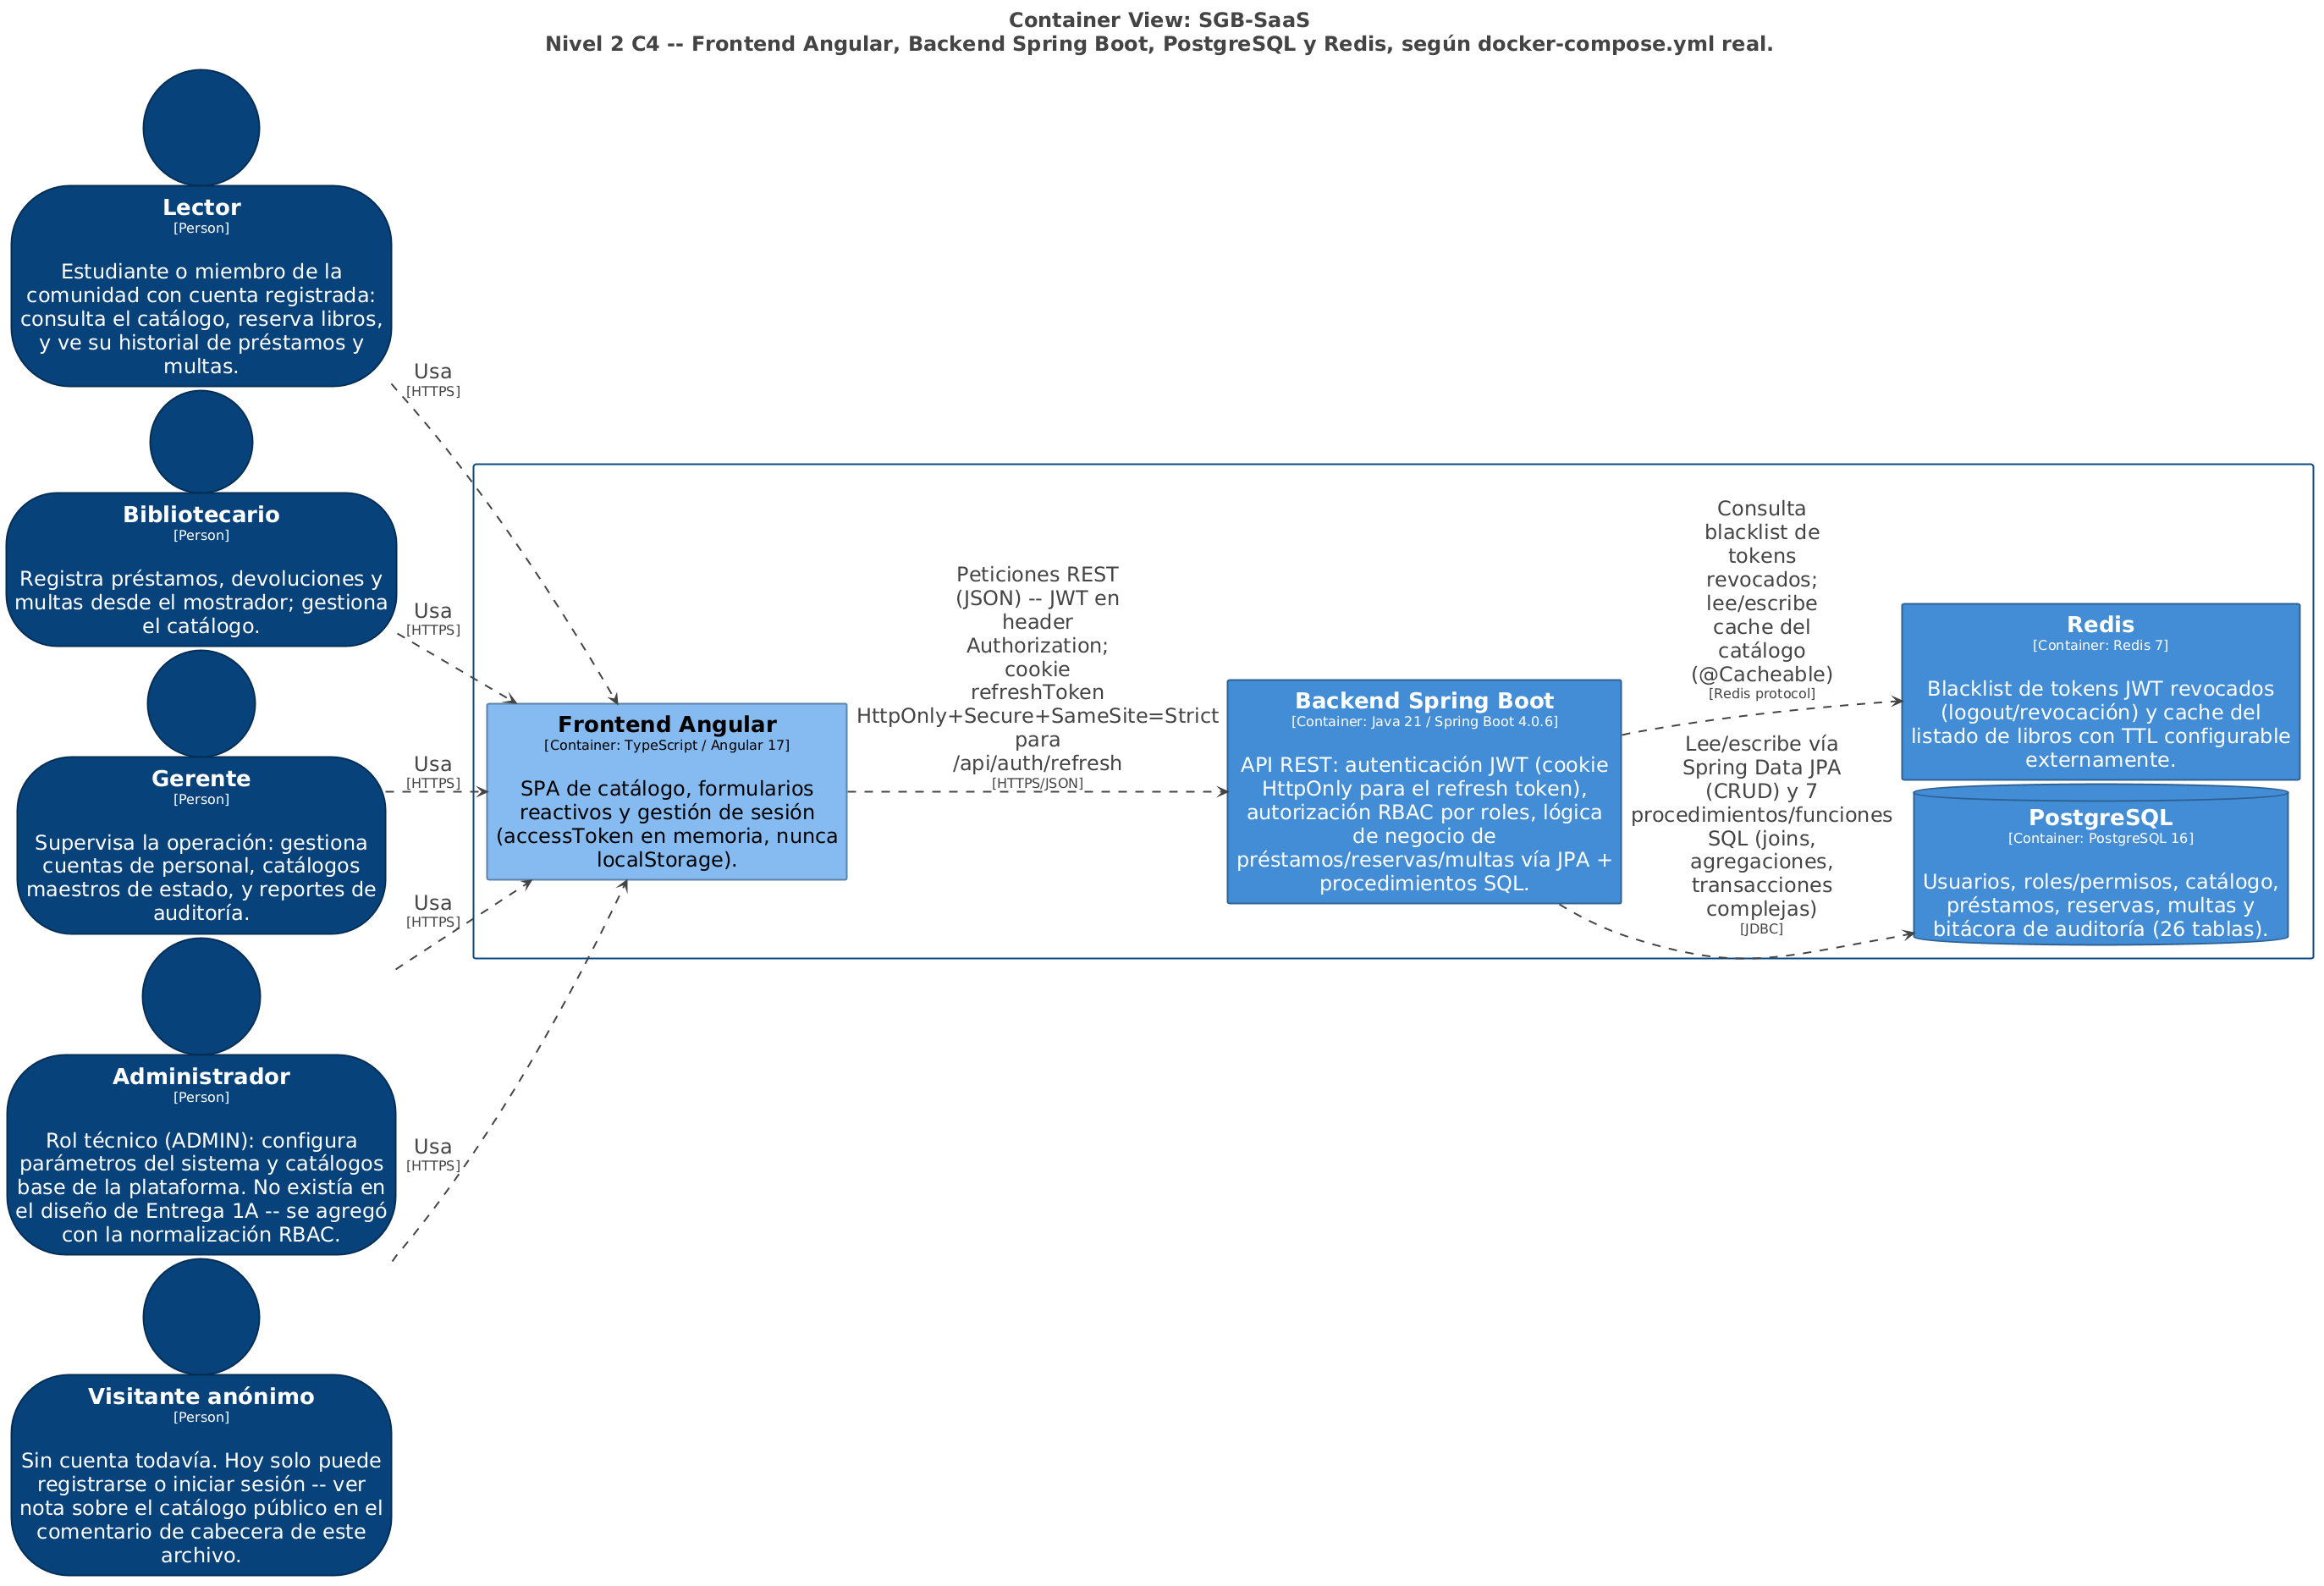
\includegraphics[width=0.95\textwidth]{arquitectura/c4-nivel2-contenedores.png}
\caption{Modelo C4, Nivel~2 (Contenedores): Frontend Angular, Backend
Spring Boot, PostgreSQL y Redis, alineados 1:1 con
\texttt{docker-compose.yml}. Exportado automáticamente desde
\texttt{workspace.dsl}.}
\label{fig:c4-nivel2-contenedores}
\end{figure}

\section{Nivel 1 -- Contexto del sistema}
\label{sec:c4-nivel1}

Cinco actores interactúan con SGB-SaaS como caja negra: \textbf{Lector}
(consulta el catálogo, reserva libros, ve su historial de préstamos y
multas), \textbf{Bibliotecario} (registra préstamos, devoluciones y
multas desde el mostrador; gestiona el catálogo),
\textbf{Gerente} (supervisa la operación: cuentas de personal, catálogos
maestros de estado y reportes de auditoría), \textbf{Administrador}
(configura parámetros del sistema y catálogos base de la plataforma --
rol que no existía en el diseño original de Entrega~1A, incorporado al
normalizar el modelo RBAC) y \textbf{Visitante anónimo} (sin cuenta
todavía; hoy solo puede registrarse o iniciar sesión).

El propio \texttt{workspace.dsl} documenta, en su comentario de
cabecera, una discrepancia real entre el diseño original de Entrega~1A y
la implementación actual que vale la pena señalar aquí: Gemini~3.5~Flash~Lite
API y Google Books API aparecían como sistemas externos en el diseño
original y se \textbf{retiraron} del diagrama actual porque no existe
ninguna integración con Google Books en el código real (Gemini sí se
integró, pero como parte interna del contenedor Backend, no como un
"sistema externo" del Nivel~1 -- ver \autoref{sec:c4-nivel3} más
abajo). Tampoco se
diseñó nunca un endpoint de catálogo público accesible sin
autenticación: \texttt{LibroController} exige rol \texttt{LECTOR} (o
superior) incluso para listar libros, así que el alcance real del
\emph{Visitante anónimo} se limita a registro e inicio de sesión.

\section{Nivel 2 -- Contenedores}
\label{sec:c4-nivel2}

Cuatro contenedores, alineados 1:1 con \texttt{docker-compose.yml}:

\begin{itemize}[leftmargin=1.2cm]
  \item \textbf{Frontend Angular} (TypeScript/Angular~21) -- SPA de
    catálogo, formularios reactivos y gestión de sesión con el
    \texttt{accessToken} en memoria, nunca en \texttt{localStorage}.
  \item \textbf{Backend Spring Boot} (Java~21/Spring~Boot~4.0.6) -- API
    REST con autenticación JWT (cookie \texttt{HttpOnly} para el
    \texttt{refreshToken}), autorización RBAC por roles, y lógica de
    negocio de préstamos/reservas/multas vía JPA y procedimientos SQL.
  \item \textbf{PostgreSQL~16} -- usuarios, roles/permisos, catálogo,
    préstamos, reservas, multas y bitácora de auditoría (26 tablas).
  \item \textbf{Redis~7} -- blacklist de tokens JWT revocados (logout /
    revocación) y caché del listado de libros con TTL configurable
    externamente.
  \end{itemize}

Respecto al diseño original de Entrega~1A, el contenedor Redis y el
actor Administrador son incorporaciones directas de la normalización
RBAC y del mecanismo de revocación de tokens vía \emph{blacklist}, ambos
ausentes del diagrama de contenedores original.

\section{Nivel 3 -- Componentes}
\label{sec:c4-nivel3}

El Nivel~3 se completó una vez cerradas las 8 ramas del módulo de
Préstamos/Reservas/Multas (evitando así reconstruir el diagrama dos
veces mientras ese módulo seguía en desarrollo activo). Se construyó a
partir del inventario real de \emph{controllers}/\emph{services}/clases
de seguridad del backend -- no del diseño aspiracional --, agrupado por
dominio en 21 componentes para mantener el diagrama legible en vez de
tener una entrada por cada una de las cerca de 30 clases reales:

\begin{itemize}[leftmargin=1.2cm]
  \item \textbf{Capa API} (7 componentes): Auth~API, Catálogo~API,
    Préstamos~API, Notificaciones~API, CredencialQR~API, Chatbot~API,
    Admin~API -- un componente por dominio funcional, no por clase
    \texttt{@RestController} individual.
  \item \textbf{Capa de servicio} (8 componentes): Auth~Service,
    Catálogo~Service, Préstamos~Service, Reportes~Service,
    Notificaciones~Service, CredencialQR~Service, Chatbot~Service, Admin
    Service.
  \item \textbf{Seguridad} (5 componentes): \texttt{JwtService},
    \texttt{JwtAuthFilter}, \texttt{UserDetailsServiceImpl},
    \texttt{LoginRateLimiter} (OWASP A07, límite de intentos de login por
    correo+IP) y \texttt{ChatbotRateLimiter} (límite de mensajes al
    asistente por usuario).
  \item \textbf{Integración externa} (1 componente): \texttt{GeminiClient}
    -- cliente HTTP hacia la API de Gemini~3.5~Flash~Lite, con reintento
    simple ante 429/timeout/5xx y sin exponer la URL con la API key en
    logs (ver ADR-016, \autoref{sec:adrs}).
\end{itemize}

Las relaciones entre componentes se verificaron contra el código real
(no se infirieron): cada flecha API~$\to$~Service, Service~$\to$~Postgres/
Redis, y las dependencias cruzadas de \texttt{ChatbotService} hacia
\texttt{CatálogoService} y \texttt{PréstamosService} para el
\emph{grounding} real de sus respuestas (consulta disponibilidad de
libros y reservas del propio usuario antes de responder, para no
inventar disponibilidad) corresponden a llamadas reales entre las
clases Java correspondientes.

\subsection*{Validación sintáctica y exportación visual}
\label{sec:c4-exportacion}

El archivo se validó sintácticamente con el motor activamente mantenido
\texttt{structurizr/structurizr} (subcomando \texttt{validate}), no con
\texttt{structurizr/cli} -- que en este momento del ecosistema
Structurizr es una imagen retirada que solo imprime un aviso de
desuso y termina con código de salida~0 para cualquier entrada, válida o
no (confirmado también al intentar el \texttt{export} con esa imagen:
código de salida~0 sin generar ningún archivo), por lo que una
validación o exportación con esa imagen no habría sido real. Los tres
niveles se exportaron con el mismo flujo activamente mantenido:
\texttt{structurizr/structurizr export -workspace workspace.dsl
-format plantuml}, seguido de renderizado con PlantUML
(\texttt{plantuml/plantuml} vía Docker). El diagrama de Nivel~3
resultó en \texttt{docs/arquitectura/c4-nivel3-componentes.svg}
(generado en una sesión previa; se confirmó en esta sesión que sigue
coincidiendo con el \texttt{workspace.dsl} vigente -- mismos 21
componentes, mismas relaciones -- por lo que no fue necesario
regenerarlo), versionado junto al DSL fuente y reproducido en la
\autoref{fig:c4-componentes}. Los diagramas de Nivel~1 y Nivel~2 se
exportaron en esta sesión de la misma forma, resultando en
\texttt{docs/arquitectura/c4-nivel1-contexto.png} y
\texttt{c4-nivel2-contenedores.png}, reproducidos en la
\autoref{fig:c4-nivel1-contexto} y la \autoref{fig:c4-nivel2-contenedores}.

\begin{figure}[h]
\centering
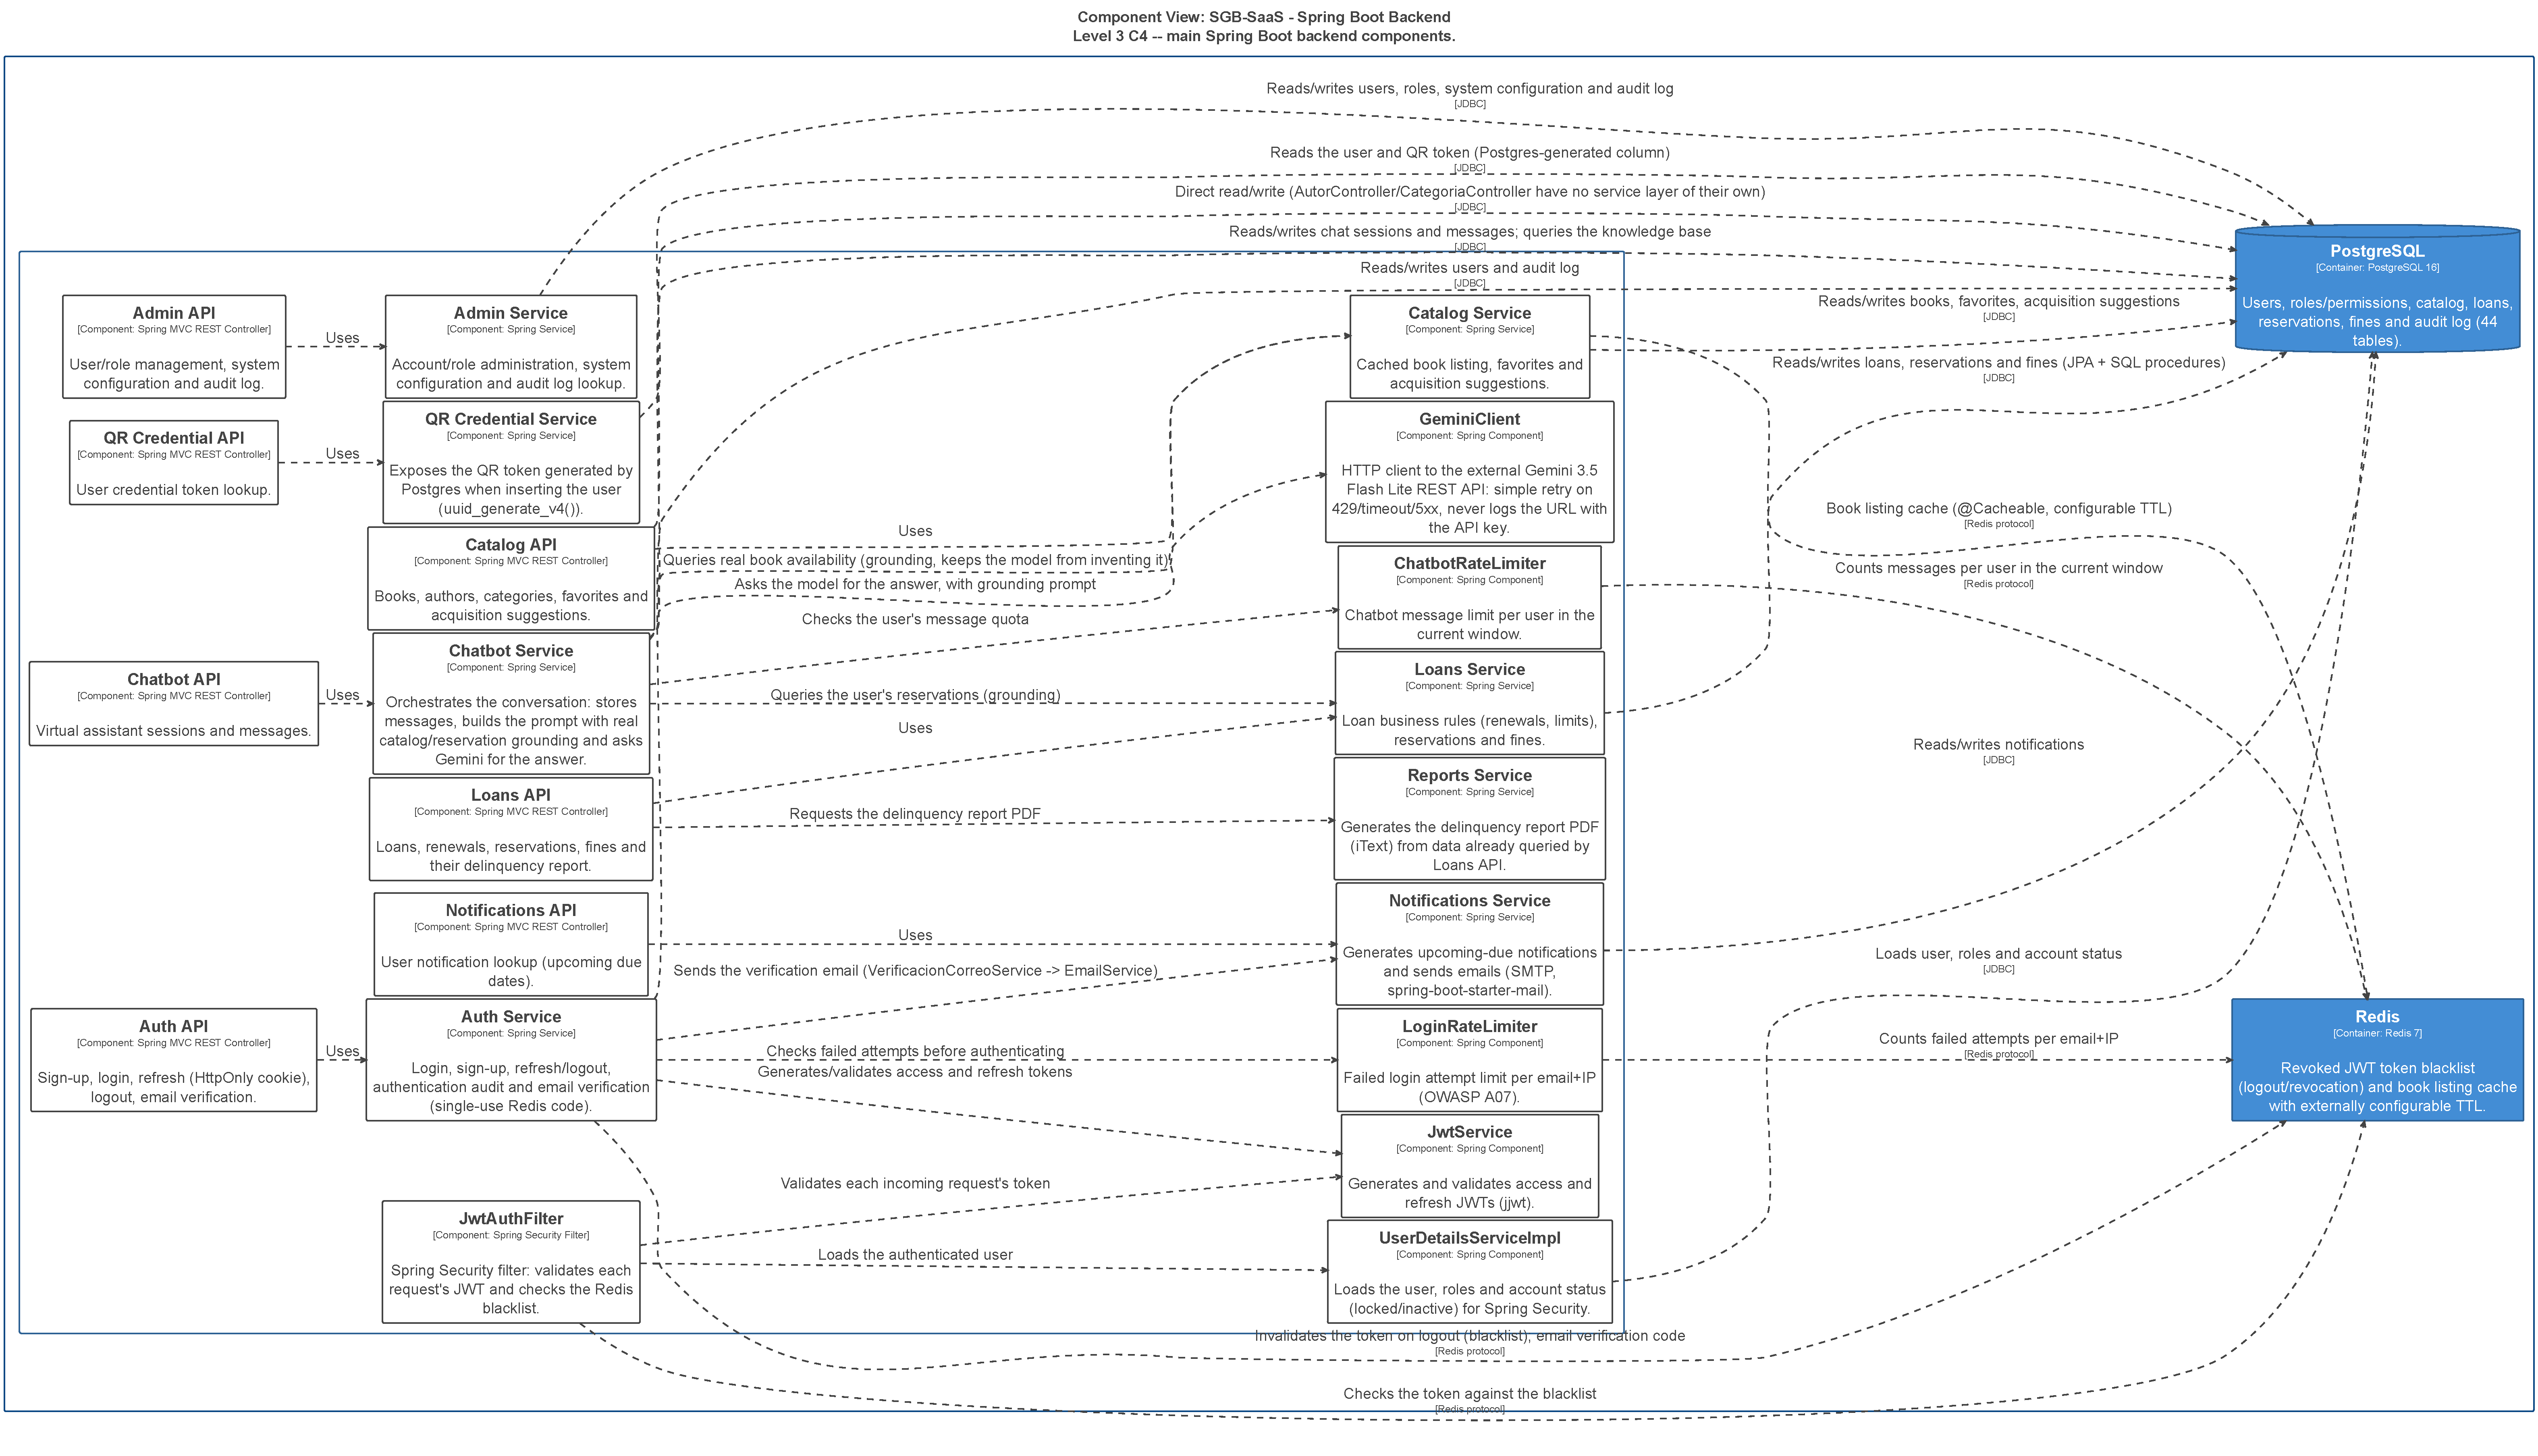
\includegraphics[width=\textwidth]{arquitectura/c4-nivel3-componentes.pdf}
\caption{Modelo C4, Nivel~3 (Componentes) del backend Spring Boot -- 21
componentes agrupados por dominio (capa API, capa de servicio,
seguridad e integración externa), con sus relaciones verificadas contra
el código real. Conversión a PDF del SVG fuente versionado en
\texttt{docs/arquitectura/c4-nivel3-componentes.svg} (pdflatex no
soporta SVG directamente).}
\label{fig:c4-componentes}
\end{figure}

\section{Decisiones arquitectónicas documentadas (ADR)}
\label{sec:adrs}

El repositorio contiene \textbf{13 Architecture Decision Records}
(\texttt{docs/adr/}), agrupados a continuación según los 6 temas
obligatorios del Bloque~D de la guía (mapeo completo en
\texttt{docs/adr/README.md}). Hasta el 26 de agosto de 2026, dos de esos
temas estaban cubiertos por un ADR cuya numeración interna del
repositorio no coincidía con la numeración sugerida por la guía
(\texttt{ADR-006}/\texttt{ADR-007} sugeridos por la guía para acceso a
datos y despliegue correspondían a \texttt{ADR-013} y \texttt{ADR-012}
en este repositorio), por continuidad con la numeración ya evaluada en
la Tercera Entrega. Se decidió renumerar de todas formas para que la
numeración coincida literalmente con la guía en vez de dejarlo como una
diferencia solo explicada en prosa -- ver la nota histórica en
\texttt{docs/adr/README.md} con el detalle del intercambio y las
referencias cruzadas actualizadas en el mismo cambio.

\begin{center}
\small
\begin{tabularx}{\linewidth}{|c|X|l|}
\hline
\rowcolor{verdeuteq}
\color{white}\textbf{\#} & \color{white}\textbf{Tema obligatorio (Bloque D)} & \color{white}\textbf{ADR(s)} \\
\hline
1 & Elección de la pila tecnológica principal & \texttt{ADR-001} \\
\hline
2 & Esquema de autenticación & \texttt{ADR-010} + \texttt{ADR-003} + \texttt{ADR-012} \\
\hline
3 & Gestor de base de datos & \texttt{ADR-011} \\
\hline
4 & Estrategia de caché & \texttt{ADR-008} \\
\hline
5 & Estrategia de despliegue & \texttt{ADR-007} \\
\hline
6 & Estrategia de acceso a datos (CRUD-ORM vs.\ SP) & \texttt{ADR-006} \\
\hline
\end{tabularx}
\end{center}

Los 7 ADR restantes no mapean a ninguno de los 6 temas obligatorios,
pero documentan decisiones reales tomadas durante el desarrollo:
\texttt{ADR-013} (versionado de esquema reproducible, Flyway + snapshot),
\texttt{ADR-009} (licencia MIT), \texttt{ADR-014} (separación de
responsabilidades entre \texttt{ADMIN} y \texttt{GERENTE}: el primero
administra permisos/configuración de plataforma, el segundo la operación
diaria -- ninguno de los dos queda excluido de \emph{ver} el padrón de
usuarios, pero solo \texttt{ADMIN} puede \emph{modificarlo}),
\texttt{ADR-015} (TLS termina en el proxy, no en el backend Spring
Boot: el backend queda preparado vía
\texttt{server.forward-headers-strategy: framework} para reconocer
\texttt{X-Forwarded-Proto} y activar HSTS el día que el proxy real
active TLS, sin cambios de código adicionales), y \texttt{ADR-016}
(qué datos exactos viajan a la API externa de Gemini en el chatbot --
texto del mensaje, historial de la sesión y un prompt de
\emph{grounding} con datos ya públicos del catálogo -- y por qué eso no
constituye una exposición indebida de información: nunca viajan
credenciales, tokens, contraseñas ni identificación personal).

\section{Atributos de calidad (ISO/IEC 25010)}

Aplicando el modelo de calidad descrito en la \autoref{sec:mt-25010},
\texttt{docs/arquitectura/ISO25010.md} prioriza las 8 características de
calidad de producto de la norma para el contexto específico de este
proyecto (biblioteca universitaria de bajo volumen, no un sistema de
alta concurrencia), citando evidencia real donde existe en vez de
estimarla. Se reproduce a continuación tal cual el documento fuente
(única fuente de verdad de esta tabla; este capítulo no la duplica de
memoria):

\begin{center}
\small
\begin{longtable}{|l|c|p{8.7cm}|}
\hline
\rowcolor{verdeuteq}
\color{white}\textbf{Característica} & \color{white}\textbf{Prioridad} & \color{white}\textbf{Estrategia / decisión que la atiende} \\
\hline
\endhead
Adecuación funcional & Alta & Procedimientos almacenados transaccionales para operaciones con lógica cruzada multi-tabla (\texttt{sp\_registrar\_devolucion}, \texttt{sp\_pagar\_multa}, \texttt{sp\_anular\_multa}), constraints de integridad referencial (FKs, CHECKs) en \texttt{db/schema.sql}. \\
\hline
Eficiencia de desempeño & Media & Caché Redis del listado de libros con TTL externo (ADR-008). Evidencia vigente: prueba de carga formal (50~VUs, 5 corridas de k6 con Wilcoxon + Cliff's delta) -- p95 agregado \textbf{19{,}49\,ms} en \texttt{cache\_caliente} (umbral $<$200\,ms) y \textbf{7{,}50\,ms} en \texttt{cache\_frio} (umbral $<$500\,ms), 0\,\% de errores 5xx en 20\,003 peticiones (\texttt{docs/mediciones/perf/REPORT.md}). El propio informe declara una limitación metodológica real (ver \autoref{cap:amenazas-validez}): \texttt{cache\_frio} mide sobre todo consultas con página vacía, no el costo real de traer una página llena sin caché. Una medición manual preliminar del 21 de julio había reportado cifras de otro orden de magnitud ($\sim$170\,ms/$\sim$30\,ms) por tratarse de una sola petición aislada sin carga concurrente; queda solo como antecedente histórico, no como evidencia vigente. \\
\hline
Compatibilidad & Media & API REST documentada con OpenAPI/Swagger vía springdoc-openapi (ADR-001), JSON como formato estándar -- sin integración real hoy con sistemas académicos institucionales ni con Google Books API. \\
\hline
Usabilidad & Alta & \texttt{sp\_registrar\_devolucion} valida el estado del préstamo antes de actuar (rechaza con \texttt{LB409} si ya estaba devuelto, evitando duplicidad); frontend Angular con formularios reactivos y validación antes de enviar. \\
\hline
Fiabilidad & Alta & Parcialmente atendida: ADR-003 documenta explícitamente que, si Redis cae, \texttt{JwtAuthFilter} queda sin forma de verificar revocaciones -- la decisión \emph{fail-open} vs.\ \emph{fail-closed} sigue anotada como pendiente para producción, no resuelta. Los \emph{healthchecks} de \texttt{docker-compose.yml} sí garantizan un orden de arranque correcto. \\
\hline
Seguridad & Alta & Cookie \texttt{HttpOnly+Secure+SameSite=None} para el \texttt{refreshToken} (ADR-012), BCrypt costo 12, blacklist de tokens revocados (ADR-003), respuestas de error RFC~7807 sin fuga de detalles internos. \textbf{Nota de este informe}\footnote{\texttt{SameSite=None} era necesario para que el navegador enviara la cookie entre los orígenes cross-origin de Render (frontend y backend en subdominios distintos), pero reintroduce la exposición a CSRF que \texttt{SameSite=Strict} bloqueaba por sí solo. El código actual tiene \texttt{.csrf(csrf -> csrf.disable())} activo (\texttt{SecurityConfig.java}, línea 55) y no implementa ningún token CSRF; el único control vigente es la lista blanca de CORS, que impide leer la respuesta cross-origin pero no impide el envío de la petición con la cookie adjunta. El ADR-012 documenta esto explícitamente como riesgo aceptado, no mitigado, con la corrección (token CSRF / \emph{double-submit cookie}) registrada como trabajo futuro (\autoref{sec:tf-csrf}).}: el diseño actual acepta explícitamente el riesgo de CSRF residual sobre \texttt{/api/auth/refresh} que introduce \texttt{SameSite=None}, según ADR-012 -- ver aclaración al pie. \\
\hline
Mantenibilidad & Alta & Los ADR de \texttt{docs/adr/} documentan decisiones no obvias con sus alternativas consideradas; \texttt{docs/basedatos/CATALOGO-SP.md} documenta el criterio de separación CRUD-ORM vs.\ procedimientos. \textbf{Nota de este informe}\footnote{El texto original de \texttt{ISO25010.md} en esta fila cita ``6 ADRs existentes'', cifra que quedó desactualizada tras incorporar los 8 módulos construidos después de la Tercera Entrega -- el repositorio contiene 13 ADRs a la fecha de este capítulo (\autoref{sec:adrs}). Se transcribe el texto original de la fuente junto con esta aclaración en vez de editarlo silenciosamente, ya que corregir \texttt{ISO25010.md} está fuera del alcance de esta tarea.}: la cifra real de ADRs es 13, no 6 -- ver aclaración al pie. \\
\hline
Portabilidad & Alta & Docker Compose con imágenes base pinadas por digest sha256, \texttt{db/init/01-consolidado.sql} generado de forma reproducible, arranque de un solo comando vía \texttt{make up}. \\
\hline
\end{longtable}
\end{center}

\section{Matriz de trazabilidad -- resumen por tipo de acceso a datos}
\label{sec:matriz-resumen}

La matriz completa de los 46 requisitos vive en
\texttt{docs/trazabilidad/matriz.csv} y se valida automáticamente en
cada ejecución de CI vía \texttt{scripts/validate-traceability.sh}. Este
capítulo no reproduce las 46 filas (el detalle completo por requisito
vive en \autoref{cap:ingenieria-requisitos} y en la propia matriz);
resume aquí la columna \texttt{tipo\_acceso}, relevante para esta
sección por ser la evidencia directa de que la estrategia híbrida
CRUD-ORM/SP declarada en ADR-006 se aplica de verdad y no solo en
teoría.

\textbf{Nota de corrección respecto a una versión anterior de este
capítulo.} \texttt{matriz.csv} tenía 4 filas
(\texttt{REQ-F-018}, \texttt{REQ-F-019}, \texttt{REQ-F-020},
\texttt{REQ-F-028}) con una coma sin escapar dentro de un campo, que
rompía el parseo CSV estándar -- defecto ya corregido en el commit
\texttt{ecfaf52}. Una versión anterior de esta tabla, calculada antes de
esa corrección, solo había detectado 2 de las 4 filas afectadas
(\texttt{REQ-F-019}, \texttt{REQ-F-020}) y las marcaba como ``sin
clasificar''; además atribuía el problema de \texttt{REQ-F-019} a la
columna \texttt{tipo\_acceso}, cuando en realidad ese campo sí tenía un
valor de \texttt{tipo\_acceso} válido (\texttt{"CRUD-ORM + generacion de
imagen (ZXing)"}) -- el campo roto en esa fila específica era
\texttt{modulo\_codigo}, no \texttt{tipo\_acceso}. Con las 43 filas
parseando limpio, la tabla de abajo reclasifica las 4 filas
correctamente en vez de dejarlas fuera:

\begin{center}
\begin{tabularx}{\linewidth}{|X|c|c|}
\hline
\rowcolor{verdeuteq}
\color{white}\textbf{Tipo de acceso a datos} & \color{white}\textbf{Requisitos} & \color{white}\textbf{\%} \\
\hline
CRUD-ORM (exclusivo, incl.\ combinado con Redis/SMTP/caché/API externa) & 21 & 48{,}8\,\% \\
\hline
Híbrido SP + CRUD-ORM (requisitos transversales) & 2 & 4{,}7\,\% \\
\hline
Procedimiento/función SQL (SP, exclusivo, incl.\ combinado con generación de PDF) & 8 & 18{,}6\,\% \\
\hline
No aplica (decisión de arquitectura, configuración, control de acceso o UI sin acceso directo a BD) & 11 & 25{,}6\,\% \\
\hline
Redis + SMTP (sin tabla Postgres nueva; no aplica CRUD-ORM ni SP)\footnote{\texttt{REQ-F-020}: \texttt{tipo\_acceso} = ``Redis (código OTP con TTL, sin tabla nueva) + SMTP (EmailService)''. Categoría propia, no un defecto de la matriz -- el código de verificación vive en Redis con TTL, sin persistirse en una tabla Postgres nueva, y el envío usa SMTP directo; no encaja limpiamente en CRUD-ORM ni en SP.} & 1 & 2{,}3\,\% \\
\hline
\textbf{Total} & \textbf{43} & \textbf{100{,}0\,\%} \\
\hline
\end{tabularx}
\end{center}

\textbf{Nota de alcance (cierre de la Entrega Final).} La matriz creció
de 43 a 46 requisitos tras esta tabla (\texttt{REQ-F-030},
\texttt{REQ-F-031}, y una extensión de \texttt{REQ-F-021} a la capa
frontend) -- los 3 no se reclasificaron en la tabla de arriba porque la
categorización por \texttt{tipo\_acceso} exige revisar el valor completo
de cada campo a mano, no solo una coincidencia de texto (ver el caso de
\texttt{REQ-F-018} más abajo, que una primera pasada automática
clasificó mal por esa misma razón); no hubo tiempo de repetir esa
revisión manual para los 3 antes del cierre. Los porcentajes de esta
tabla y del párrafo siguiente siguen describiendo, con honestidad, la
distribución de los 43 requisitos originales, no los 46 vigentes.

De los 43 requisitos originales de esta tabla, 10 (23{,}3\,\%) involucran al menos un
procedimiento o función SQL (8 exclusivamente, 2 en combinación con
CRUD-ORM: \texttt{REQ-NF-004}, transversal a los módulos de
préstamos/multas/reservaciones vs.\ auth/libros/bitácora, y
\texttt{REQ-NF-013}, prevención de inyección SQL sobre ambos
mecanismos), consistente con la justificación de ADR-006: reservar los
procedimientos almacenados para operaciones con validación cruzada
multi-tabla o transacciones atómicas compuestas (registrar préstamo,
registrar devolución, pagar multa, anular multa, expirar reservaciones
vencidas, y los 3 reportes agregados), dejando el CRUD elemental de una
sola tabla en Spring Data JPA. \texttt{REQ-F-018} (renovación de
préstamo), pese a mencionar textualmente ``SP'' en su valor de
\texttt{tipo\_acceso} (``CRUD-ORM (validación en Java, sin SP nuevo)''),
es CRUD-ORM exclusivo: la frase aclara explícitamente que la renovación
\emph{no} introdujo un procedimiento almacenado nuevo, la validación de
sus 3 reglas de negocio corre en Java -- se señala aquí porque una
primera pasada de clasificación automática por coincidencia de texto
la contó por error como híbrida, hasta revisar el valor completo del
campo.
